\documentclass[slidestop,compress,blackandwhite]{beamer}

\usepackage[utf8x]{inputenc}
\usepackage[italian]{babel}
\usepackage{tikz}
\usepackage{nameref}

\usetheme{Antibes}
\usecolortheme{default}


\pgfdeclareimage[height=1.5cm]{logo}{imgs/unipd_logo}

\setbeamercolor{block title}{fg=red,bg=structure!15}

\setbeamercolor{block body}{bg=structure!15}

% TITOLO
\setbeamercovered{transparent}

\author{Moreno Ambrosin}

\title[Progetto esame di Sistemi Concorrenti e Distribuiti]{Railway Simulation}

\institute[\insertframenumber/\inserttotalframenumber]{
	\large{Università degli studi di Padova} \\
	\vspace{5pt}
	\normalsize Facoltà di Scienze MM. FF. NN. \\
	\vspace{5pt}
	\small Corso di laurea in Informatica
}
\date{Settembre 2013}

\newcommand{\itemB}[3]{
	\item \textbf{#1} #2 \vspace{#3}
}

\newcommand{\ttt}[1]{\texttt{#1}}
\newcommand{\ii}[1]{\textit{#1}}

\newcommand{\treno}{\ii{treno}}
\newcommand{\treni}{\ii{treni}}
\newcommand{\viaggiatore}{\ii{viaggiatore}}
\newcommand{\viaggiatori}{\ii{viaggiatori}}
\newcommand{\stazione}{\ii{stazione}}
\newcommand{\stazioni}{\ii{stazioni}}
\newcommand{\piattaforma}{\ii{piattaforma}}
\newcommand{\piattaforme}{\ii{piattaforme}}
\newcommand{\binario}{\ii{binario}}
\newcommand{\binari}{\ii{binari}}
\newcommand{\ticket}{\ii{biglietto}}
\newcommand{\tickets}{\ii{biglietti}}
\newcommand{\segmento}{\ii{segmento}}
\newcommand{\segmenti}{\ii{segmenti}}
\newcommand{\route}{\ii{percorso}}
\newcommand{\routes}{\ii{percorsi}}
\newcommand{\stage}{\ii{tappa}}
\newcommand{\stages}{\ii{tappe}}
\newcommand{\biglietteria}{\ii{biglietteria}}
\newcommand{\biglietterie}{\ii{biglietterie}}
\newcommand{\timetable}{\ii{tabella oraria}}
\newcommand{\timetables}{\ii{tabelle di orari}}
\newcommand{\controller}{\ii{controllo centrale}}
\newcommand{\regione}{\ii{regione}}
\newcommand{\regioni}{\ii{regioni}}
\newcommand{\gateway}{\ii{stazione di gateway}}
\newcommand{\gateways}{\ii{stazioni di gateway}}

\newcommand{\PRO}{\textbf{PRO:}}
\newcommand{\CONTRO}{\textbf{CONTRO:}}

\newcommand{\newtitle}[4]{
	#1 
	\ifx&#2&%
	\else
  		\large- #2
	\fi
	\ifx&#3&%
	\else
  		\normalsize- #3
	\fi
	\ifx&#4&%
	\else
  		\normalsize (#4)
	\fi
}

\newcommand{\newframe}[5]{
	\begin{frame}
		\frametitle{\newtitle{#1}{#2}{#3}{#4}}
		#5
	\end{frame}
}

\newcommand{\itemt}[1]{\item (\ttt{#1})}
\newcommand{\myitemize}[1]{\begin{itemize}#1\end{itemize}}

\begin{document}
	
	\usebackgroundtemplate{
		\hspace{0.13\paperwidth}
\includegraphics[height=\paperheight]{imgs/logoUnipd}
	}	
	
	\begin{frame}[c]
		\titlepage
	\end{frame}
	
%	\logo{\pgfuseimage{logo}}
	
%	\usebackgroundtemplate{}
	
	\begin{frame}
		\frametitle{Indice}
		\tableofcontents
	\end{frame}
	
	\setbeamertemplate{footline}[text line]{\parbox{\linewidth}{\vspace*{-8pt}\insertframenumber/\inserttotalframenumber\hfill Progetto Sistemi Concorrenti e Distribuiti\hfill}}
	
	\section{Il Problema}
	\subsection{Descrizione}
	
	\newframe{Descrizione}{}{}{}{
		Simulatore software concorrente e distribuito, per la simulazione di un sistema ferroviario composto da:
		\begin{itemize}
			\item \treni, appartenenti a diverse categorie.
			\item \viaggiatori, che operano azioni elementari come acquisto di \tickets, salita a bordo e discesa dai treni, attesa presso il \binario.
			\item \stazioni~composte da 
				\begin{itemize}
					\item \binari~interni di sosta per i \treni;
					\item \piattaforme~di attesa per i \viaggiatori;
					\item una \biglietteria~interna, accessibile ai \viaggiatori;
					\item un \ii{pannello informativo}.
				\end{itemize}
			\item \segmenti~che collegano le diverse \stazioni.
			\item un \controller~che mantiene lo stato di ciascun \treno~e di ciascun \viaggiatore~in transito.
		\end{itemize}
	}
	
	\subsection{Requisiti di alto livello}\label{requirements}
	
	\newframe{\nameref{requirements}}{}{}{1}{
		\textbf{Treno}
		\begin{itemize}
			\itemt{RT1} Ciascun \treno, appatiene ad una delle seguenti categorie: \ttt{FB} o \ttt{REG}.
				\begin{itemize}
					\itemt{RT1.1} La categoria \ttt{FB} ha priorità più alta rispetto a \ttt{REG} nell'accesso a \stazione, \piattaforme~e \binari.
				\end{itemize}
			\itemt{RT2} Ciascun \treno~è caratterizzato da un identificativo univoco, e possiede capacità e velocità massime, e mantiene stazioni di partenza e destinazione.
			\itemt{RT3} Ciascun \treno~effettua continuamente un tragitto simmetrico di andata e ritorno, definito da un \route~costituito da più \stages
				\begin{itemize}
					\itemt{RT3.1} Il tragitto di ciascun \treno~è scandito da una \timetable, che definisce,per ciascuna \stage, l'orario di partenza.
				\end{itemize}
		\end{itemize}
	}
	
	
	\newframe{\nameref{requirements}}{}{}{2}{
	
		\begin{itemize}
			\item[]
			\begin{itemize} 
				\itemt{RT3.2} Ciascuna \stage~definisce:
				\begin{itemize}
					\item \stazioni~di partenza e destinazione
					\item \piattaforme~di partenza e destinazione
					\item azione da compiere all'arrivo presso la destinazione, tra \ttt{STOP} e \ttt{PASS}
					\item il prossimo \segmento~da utilizzare.
				\end{itemize}
			\end{itemize}
			\itemt{RT4} I \treni~di tipo \ttt{FB} sono a prenotazione.
		\end{itemize}
		\vspace{0.5cm}
		\textbf{Viaggiatore}
		\begin{itemize}
			\itemt{RV1} Ciascun \viaggiatori~possiede una \stazione~di partenza ed una di destinazione.
			\itemt{RV2} Per poter salire a bordo di un \treno, ciascun \viaggiatori~deve prima acquistare un \ticket~presso la \biglietteria~della \stazione~di partenza.
		\end{itemize}
	}

	\newframe{\nameref{requirements}}{}{}{3}{
		\begin{itemize}
			\itemt{RV3} Una volta arivato a destinazione, ciascun \viaggiatore~attende un tempo casuale prima di ritornare alla stazione di partenza.
			\itemt{RV4} Il viaggio di ciascun \viaggiatore~può comprendere cambi di \treno.
		\end{itemize}
		\vspace{0.5cm}
		\textbf{Segmento}
		\begin{itemize}
			\itemt{RS1} Ciascun \segmento~è ha un identificativo univoco, una lunghezza e una velocità massima di percorrenza; esso collega esattamente due \stazioni~diverse.
			\itemt{RS2} Un \segmento~ha percorrenza bidirezionale; inoltre più \treni~possono percorrere il \segmento~nello stesso senso di marcia (percorrenza multipla).  
		\end{itemize}
	}

	\newframe{\nameref{requirements}}{}{}{4}{
		\vspace{0.5cm}
		\textbf{Stazione}
		\begin{itemize}
			\itemt{RST1} Ciascuna \stazione~è caratterizzata da un identificativo univoco.
			\itemt{RST2} Ciascuna \stazione~contiene:
				\begin{itemize}
					\item Un certo numero $N$ di \binari~di sosta per i \treni, a percorrenza bidirezionale e ad accesso mutuamente esclusivo.
					\item Un certo numero $N$ di \piattaforme~per l'attesa dei passeggeri.
					\item Un \ii{pannello informativo} che riporta informazioni su \treni~in arrivo, in transito, e che hanno appena superato la \stazione.
					\item Una biglietteria accessibile ai \viaggiatori, per l'acquisto del biglietto necessario.
				\end{itemize}
		\end{itemize} 
	}

%###################################### DISTRIBUZIONE	

	\section{Distribuzione}
	
	\subsection{Caratteristiche desiderabili}\label{characteristics}
	\newframe{\nameref{characteristics}}{}{}{}{
		\begin{itemize}
			\itemB{Distribution Transparency}{}{1cm}
			\itemB{Openess}{}{1cm}
			\itemB{Scalability}{}{1cm} 
		\end{itemize}
	}
	
		
	\newframe{\nameref{characteristics}}{Distribution Transparency}{}{}{
		
		Il sistema appare all'utilizzatore come un sistema monolitico.
		\begin{itemize}
			\item Deve fornire un unico metodo per accedere alle risorse (\ii{Access Transparency}).
			\item Deve nascondere all'utente la locazione fisica delle risorse (\ii{Location Transparency}) e la loro migrazione (\ii{Migration Transparency}).
			\item Deve nascondere all'utilizzatore finale la possibilità che le risorse siano replicate (\ii{Replication Transparency}).
			\item Deve nascondere all'utente l'eventuale accesso concorrente ad una stessa risorsa condivisa (\ii{Concurrency Transparency}).
			\item Deve rendere il sistema trasparente rispetto ai malfunzionamenti (\ii{Faliure Transparency}).
		\end{itemize}
		
		Il grado di trasparenza da adottare dipende dal problema.
	}
	
	
	\newframe{\nameref{characteristics}}{Openess}{}{}{
		Il sistema deve essere fruibile mediante un'interfaccia semplice.
		
	}

	
	\subsection{Scelete progettuali}\label{scelte}
	
	\newframe{\nameref{scelte}}{}{}{}{
		
		Il grado di distribuzione da utilizzare va scelto con cura.
		\begin{itemize}
			\item Pro e contro per diverse soluzioni possibili.
			\item Analisi delle implicazioni.
		\end{itemize}
		
		Analisi di tre soluzioni a grado di distribuzione diverso. 
		
	}
	
	\subsection{Soluzione A}
	
	\newframe{Soluzione A}{Descrizione}{}{1}{
		Primalla Soluzione valutata: tutte le entità risiedono su un diverso nodo di calcolo.
		\begin{itemize}
			\item Ciascuna \stazione, \treno~e \viaggiatore~esegue su uno specifico nodo di calcolo.  
			\item Le \stazioni~espongono un'interfaccia remota per l'iterazione con \treni~e \viaggiatori.
			\item Unica entità \biglietteria, accessibile ai \viaggiatori~tramite interfaccia esposta dalle \stazioni.
			\item Unice entità di \controller, che espone interfaccia remota a \treni~e \stazioni.
			\item Server dei nomi presso il quale le entità si registrano all'avvio del sistema.
		\end{itemize}
	}
	
	\newframe{Soluzione A}{Descrizione}{}{2}{
		\begin{figure}
			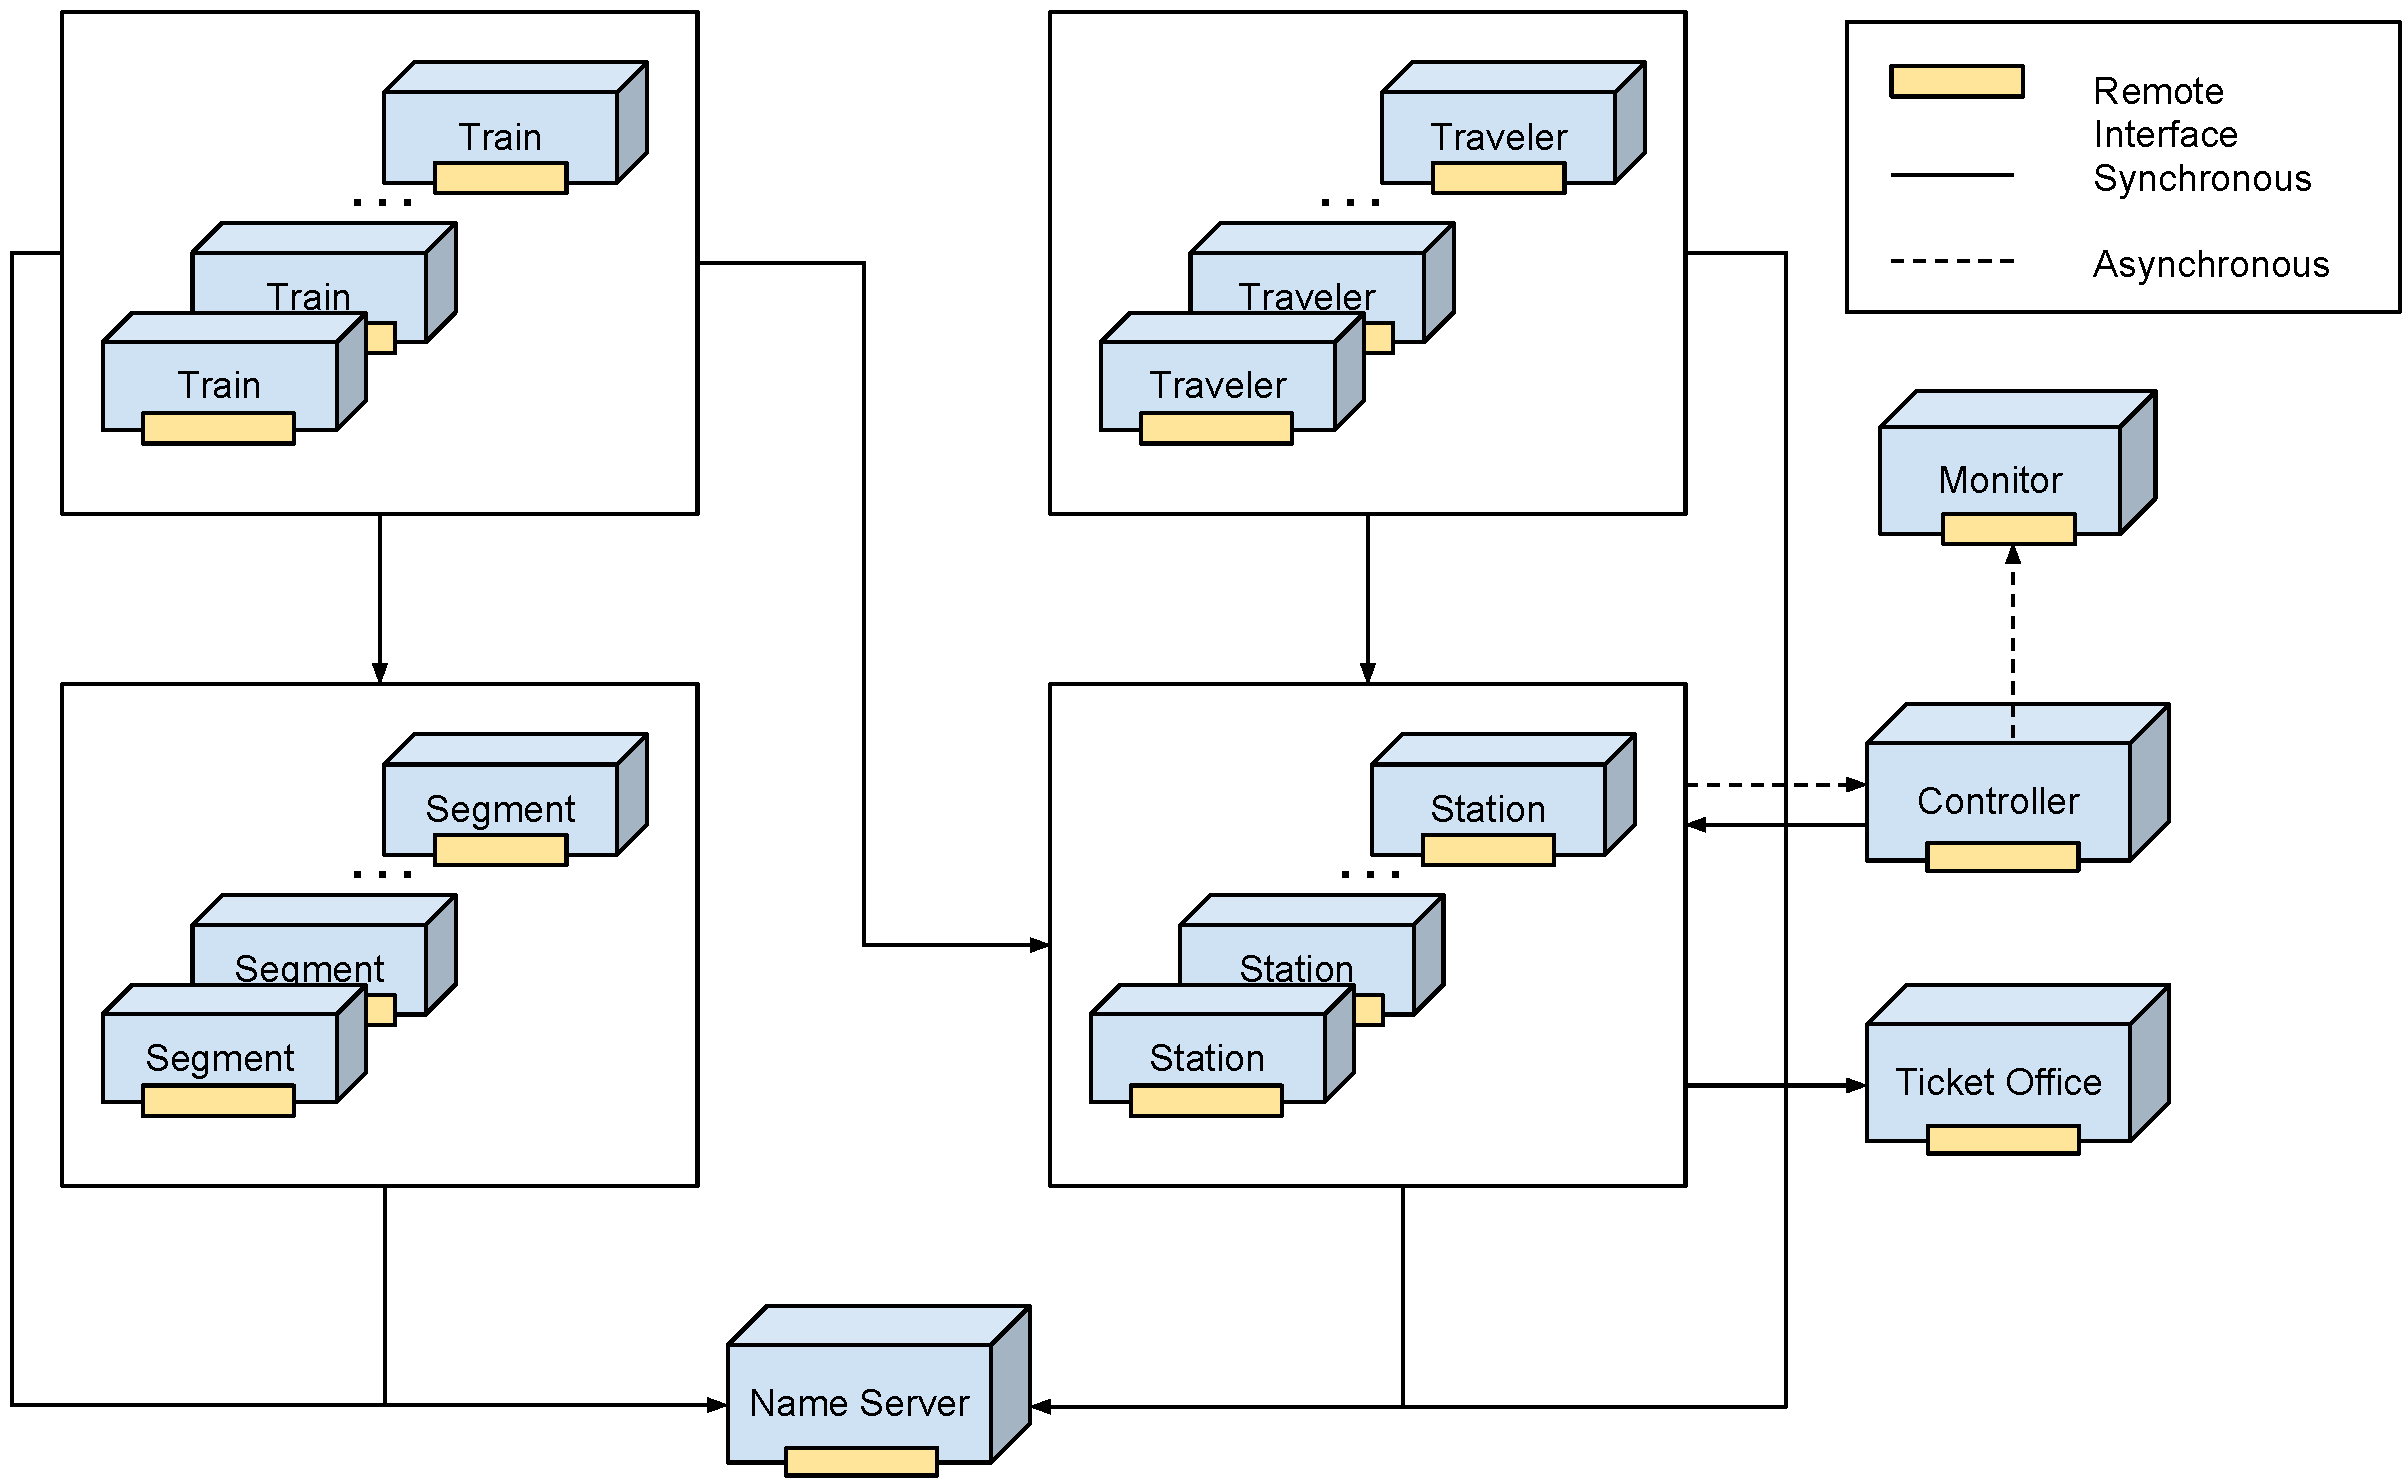
\includegraphics[scale=0.24,trim=0mm 5mm 0mm 20mm]{imgs/All_distributed.pdf}
			\caption{\small{Grafico informale che illustra l'architettura di distribuzione di massima dellalla Soluzione presentata.}}
		\end{figure}
	}
	
			
	
	\newframe{Soluzione A}{Valutazione}{}{1}{
		\PRO
			\begin{itemize}
				\item Sistema scalabile in dimensione rispetto a \treni, \stazioni~e \viaggiatori.
				\item Robusto rispetto a malfunzionamenti di \treni, \stazioni~e \viaggiatori, con impatto ridotto sull'intero sistema.
%				\item Guadagno in termini di \ii{Location Transparency}.
				\item \ii{Distribution Transparency} rispetto alle entità \ii{Monitor}.
			\end{itemize}
		
	}

	\newframe{Soluzione A}{Valutazione}{}{2}{
		\CONTRO
			\begin{itemize}
				\item Sincronizzazione in distribuito.
				\item Differenza tra i clock fisici delle macchine che compongono il sistema possono creare inconsistenze.
				\item La \biglietteria~deve mantenere tutta l'informazione relativa alla topologia del sistema ferroviario, e allo stato di prenotazione dei \treni.
				\item Rischio di comunicazioni errate, a causa dell'inaffidabilità della rete; conseguente perdita di performance. 
				\item Elevato traffico di rete.
				\item Terminazione e avvio del sistema complesse.
			\end{itemize}
	}
	
	\subsection{Soluzione B}
	\newframe{Soluzione B}{Descrizione}{}{1}{
		Secondalla Soluzione valutata: entità di simulazione in un unico nodo di calcolo.
		\begin{itemize}
			\item Solo \controller~e \ii{monitor} distribuiti.
		\end{itemize}
		
		\begin{figure}
			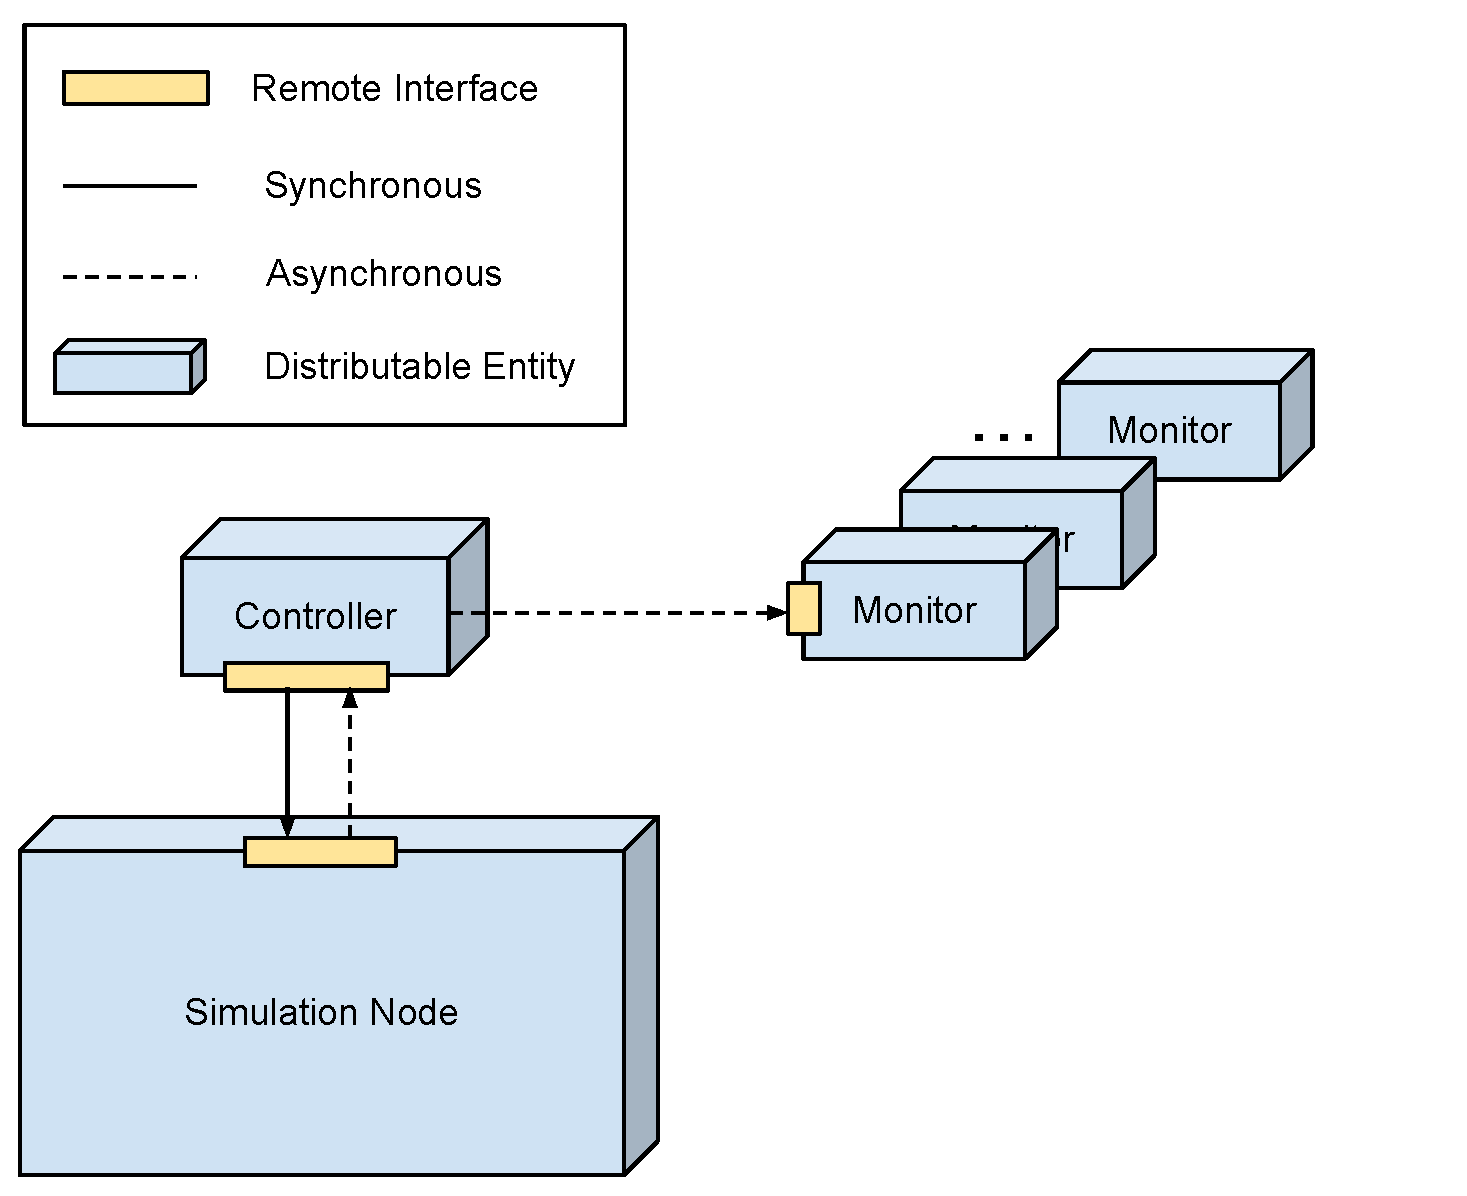
\includegraphics[scale=0.22,trim=0mm 5mm 0mm 0mm]{imgs/nothing_distributed.pdf}
			\caption{\small Grafico informale che illustra l'architettura di distribuzione di massima dellalla Soluzione presentata.}
		\end{figure}
		
	}
	
	\newframe{Soluzione B}{Valutazione}{}{1}{
		\vspace{0.5cm}
		\PRO
			\begin{itemize}
				\item Seplicità implementativa.
				\item Interazione tra entità risolta in locale mediante meccanismi di concorrenza.
				\item Utilizzo di un unico riferimento temporale; assenza di inconsistenze dovute a clock fisici non sincronizzati.
				\item Semplicità di Avvio e Terminazione dell'intero sistema.
				\item Comunicazione tra le entità di simulazione affidabili.
				\item Traffico di rete minimo.
			\end{itemize}
	}
	
	
	\newframe{Soluzione B}{Valutazione}{}{1}{
		\vspace{0.5cm}
		\CONTRO
			\begin{itemize}
				\item Di scarso interesse.
				\item Fragile rispetto a malfunzionamenti.
				\item Non scalabile.
				\item Conoscenza su Topologia e Stato in un unico luogo.
				\item Carico computazionele elevato sul singolo nodo di simulazione.
			\end{itemize}
	}
	
	\subsection{Soluzione Adottata}
	
	\newframe{Soluzione Adottata}{Descrizione}{}{1}{
		\vspace{0.5cm}
		\begin{itemize}
			\item Soluzione intermedia che mitiga le problematiche riscontrate nelle Soluzioni A e B.
			\item Introduzione di \regioni~per distribuire il carico computazionale su nodi diversi
			\item Ciascuna \regione~risiede su un proprio nodo di calcolo.
			\item In ciascuna \regione~vi sono un certo numero di \stazioni, di \segmenti, di \treni~e di \viaggiatori.
			\item Necessario l'utilizzo di un \ii{Server dei Nomi} per lookup degli indirizzi delle varie \regioni.
		\end{itemize}
	
	}
	
	\newframe{Soluzione Adottata}{Descrizione}{}{2}{
		\vspace{0.5cm}
		\myitemize{
			\item Introduzione di più livelli di \biglietterie:
				\myitemize{
					\item \ii{interne alle stazioni:} Forniscono da interfaccia per accedere alle biglietterie regionali.
					\item \ii{regionali:} Hanno conoscenza della topologia interna a ciascuna regione; si occupano della creazione dei \tickets.
					\item \ii{centrale:} Mantiene lo stato di prenotazione dei \treni~\ttt{FB}
				}
			\item L'entità di \controller~è centralizzata, e raccoglie lo stato della simulazione; esso si occupa inoltre delle procedure di Avvio e Terminazione del sistema.
		}
	}
	
	\newframe{Soluzione Adottata}{Valutazione}{}{1}{
		\vspace{0.5cm}
		\PRO
		\begin{itemize}
			\item L'utilizzo delle \regioni~è un buon compromesso per controllare la complessità del sistema.
			\item Il sistema è scalabile rispetto alla dimensione.
			\item Distribuisce la conoscenza relativa alla topologia del sistema ferroviario a livello di regioni (non più centralizzata).
			\item La \biglietteria~centrale mantiene solo lo stato relativo alle prenotazioni dei \treni~\ttt{FB}.
		\end{itemize}
	
	}
	
	\newframe{Soluzione Adottata}{Valutazione}{}{2}{
		\vspace{0.5cm}
		\CONTRO
		\begin{itemize}
			\item Rimane il problema dei clock fisici non sincronizzati, anche se con impatto minore rispetto alla Soluzione A.
			\item Maggiore complessità di Avvio e Terminazione del sistema rispetto alla Soluzione B.
			\item Meno robusta ai fallimenti rispetto alla Soluzione A .
			\item Maggiore traffico di rete rispetto alla Soluzione B
		\end{itemize}
	}
	
	\newframe{Soluzione Adottata}{Requisiti}{}{}{
		\vspace{0.5cm}
		\textbf{Requisiti aggiuntivi}
		\begin{itemize}
			\itemt{RT5} I \treni~possono compiere tragitti che attraversano più \regioni.
			\itemt{RV5} I \viaggiatori~possono viaggiare attreverso più \regioni.
		\end{itemize}
	}
	
	\newframe{Soluzione Adottata}{Problematiche}{}{}{
		\vspace{0.5cm}
		\begin{enumerate}
			\item Come rappresentare il trasferimento di \treni~e \viaggiatori~tra \regioni? 
			\vspace{0.4cm}
			\item Come gestire le problematiche relative al tempo?
			\vspace{0.4cm}
			\item Come organizzare avvio e terminazione del sistema?
		\end{enumerate}
	}
	
	\newframe{Soluzione Adottata}{Problematiche}{Trasferimento remoto}{1}{
		\vspace{0.5cm}
		\myitemize{
			\item Sono introdotte \gateways.
			\item Luogo unico dal quale i \treni~possono uscire dalla regione corrente e accedere a un'insieme di \regioni.
			\item Una volta che un \treno~accede ad una \gateway~e viene trasferito su una regione $R'$, esso riprenderà il suo \route~dalla \gateway~corrispondente presso $R'$. 
		}
	}
	
	\newframe{Soluzione Adottata}{Problematiche}{Trasferimento remoto}{2}{
		\vspace{0.5cm}
		\myitemize{
			\item Sono posti dei vincoli sull'utilizzo di \gateways:
				\myitemize{
					\item Siano $g$ ed $g'$ \gateways~appartenenti rispettivamente a due \regioni~$R$ ed $R'$. Allora se da $g$ è possibile raggiungere $g'$ in modo diretto (e viceversa), allora $!\exists g''$ appartenente a $R$ tale per cui da $g''$ si può raggiungere $g'$.\\
					$\Rightarrow$ In questo modo, dal punto di vista dei \treni, $g$ e $g'$ saranno la stessa \stazione~logica.
				
				}
		}
	}
	
	\newframe{Soluzione Adottata}{Problematiche}{Trasferimento remoto}{3}{
		\vspace{0.5cm}
		\myitemize{
			\item[] 
				\myitemize{
					\item I \binari di sosta per i \treni, interni a ciascuna \gateway, sono unidirezionali. Inoltre, ciascuna \gateway~avrà $p_1,p_2,...,p_m$ \binari~per permettere l'uscita dalla \regione corrente, e $p_{m+1},p_{m+2},...,p_k$ \binari~per consentire l'arrivo dei \treni provenienti da altre stazioni. I \binari~$p_1,p_2,...,p_m$ avranno il loro corrispettivo presso le altre \gateways~connesse per permettere l'arrivo dei treni provenienti dalla \regione~corrente. Il numero di \binari (e \piattaforme) date  $g_1,g_2,...,g_n$ \gateways, è $sum_{i=1}^{n} m_i$.\\
						$\Rightarrow$ Questo permette di mantenere locale alle regioni la competizione per l'accesso al \binario.	
				}
		}	
	}	
		
\end{document}

